\documentclass[10pt]{article}
\usepackage[a4paper,margin=1.6cm,top=1.3cm,bottom=1.3cm]{geometry}
\usepackage[T1]{fontenc}
\usepackage{lmodern}
\usepackage{microtype}
\usepackage{booktabs}
\usepackage{graphicx}
\usepackage{enumitem}
\usepackage{xcolor}
\usepackage[colorlinks=true,linkcolor=black,citecolor=black,urlcolor=blue]{hyperref}
\setlist{nosep,leftmargin=1.2em,topsep=1pt}
\setlength{\parindent}{0pt}
\setlength{\parskip}{3pt}
\pagestyle{empty}
\newcommand{\head}[1]{\par\smallskip{\large\bfseries #1}\par}
\newcommand{\sect}[1]{\par\smallskip{\bfseries\color{black!80} #1}\par}

\begin{document}
\head{Idea 5 PoC --- A machine benchmark for Chinese analysts}
\textit{Proof of concept, October 2026. Code: \texttt{idea05\_ml\_analyst\_bias/run.py}.}

\sect{Question and design}
Are Chinese consensus forecasts biased \emph{conditionally}, relative to a look-ahead-free machine forecast? Does
that bias predict returns, and with the negative US sign (van Binsbergen et al., 2023) or the positive sign reported for China
(Liu et al., 2023)? The forecast is the I/B/E/S 12-month-forward consensus scaled by price, $F_m$. The outcome is
the I/B/E/S trailing EPS twelve months later scaled by the same price, $R_m$. Keeping the outcome inside I/B/E/S
avoids the bonus-share basis mismatch with the quarterly EPS. An XGBoost model predicts $R_m$ from public data
only: trailing EPS/P, B/M, size, past returns, turnover, the latest surprises and streak, and TTM EPS growth. It is
retrained every January, using only rows whose outcome had already been realised. Conditional bias is
$F_m-\widehat{R}^{ML}_m$. Test sample: 181{,}482 covered firm-months, 2,860 firms, 2009--2020.

\begin{center}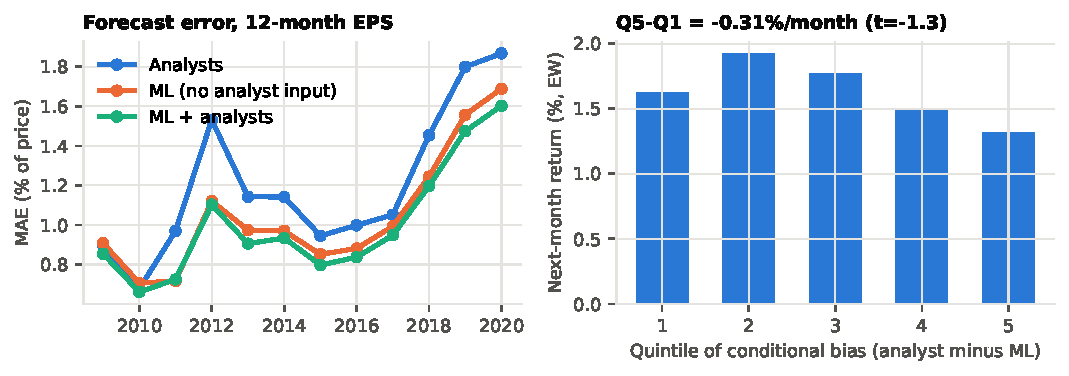
\includegraphics[width=0.97\textwidth]{results/fig_main.pdf}\end{center}

\begin{center}\small
\begin{tabular}{lccc}
\toprule
 & Analysts & ML, no analyst input & ML + analysts\\
\midrule
MAE (\% of price) & 1.19 & 1.02 & 0.98\\
Mean error $R-f$ (\% of price) & $-0.66$ & $-0.05$ & $-0.06$\\
Share of firm-months beating analysts & -- & 54.9\% & 58.1\%\\
\bottomrule
\end{tabular}\\[4pt]
\begin{tabular}{lcccc}
\toprule
Bias quintile portfolios (next month) & Q5$-$Q1 raw & CH-3 $\alpha$ & CH-4 $\alpha$ & FM slope per 1 SD of bias\\
\midrule
Equal-weighted & $-0.31$ ($-1.3$) & $-0.71$ ($-2.6$) & $-0.83$ ($-3.0$) & $-0.15$ ($-3.0$)\\
Value-weighted & $-0.18$ ($-0.5$) & $-0.41$ ($-1.1$) & $-0.59$ ($-1.7$) & \\
\bottomrule
\end{tabular}\\[2pt]
{\footnotesize \% per month ($t$-statistics, Newey--West). The FM regression controls for size, B/M, momentum,
short-term reversal and turnover.}
\end{center}

\sect{Findings}
\begin{itemize}
\item \textbf{A simple machine beats the consensus.} Without seeing any analyst input, XGBoost lowers the MAE by
  14\% and is more accurate in every year from 2011. Adding the consensus as an input helps further, so analysts do
  carry information the model lacks (``man + machine'').
\item \textbf{Analysts are optimistic, and predictably so.} The consensus exceeds the realised outcome by 0.66\% of
  price on average, while the machine is almost unbiased. The conditional bias predicts the analyst error almost
  one for one (slope $-0.87$, $t=-12.7$).
\item \textbf{Optimism relative to the machine predicts \emph{lower} returns, as in the US.} Stocks with the most
  optimistic analysts underperform by 0.83\% per month on a CH-4 basis (EW). The FM slope is negative after
  standard controls. This is the opposite of the positive sign Liu et al.\ (2023) report with a statistical
  benchmark. The effect is weaker value-weighted and after 2015.
\end{itemize}

\sect{Caveats and next steps}
(i) The panel holds only the time-weighted 12-month consensus, and the trailing ``outcome'' partly blends in later
forecasts. Fiscal-year I/B/E/S detail (FY1 and FY2 consensus with the number of analysts) would give a clean
target. (ii) The raw spread is insignificant; the alpha comes from factor loadings, so the risk adjustment needs
scrutiny. (iii) Next: reconcile with Liu et al.\ by replicating their growth-forecast signal on the same sample,
and check the look-ahead discipline that Zhang et al.\ (2025) show can reverse US conclusions.

{\footnotesize \textbf{References.} van Binsbergen, Han and Lopez-Lira (2023, RFS); Zhang, Zhu and
Linnainmaa (2025, RFS); Liu, Zhu, Zhang and Zhang (2023, PBFJ); Campbell, Ham, Lu and Wood (Management Science,
forthcoming).}
\end{document}
